\section{Anden iteration}

\subsection{Transformator}
Figur~\ref{fig: Primarinduktans} viser induktansen målt i transformatorens primærvikling, ved et frekvenssweep $100Hz$ til $1MHz$.. 
\begin{figure}[H]
	\center
	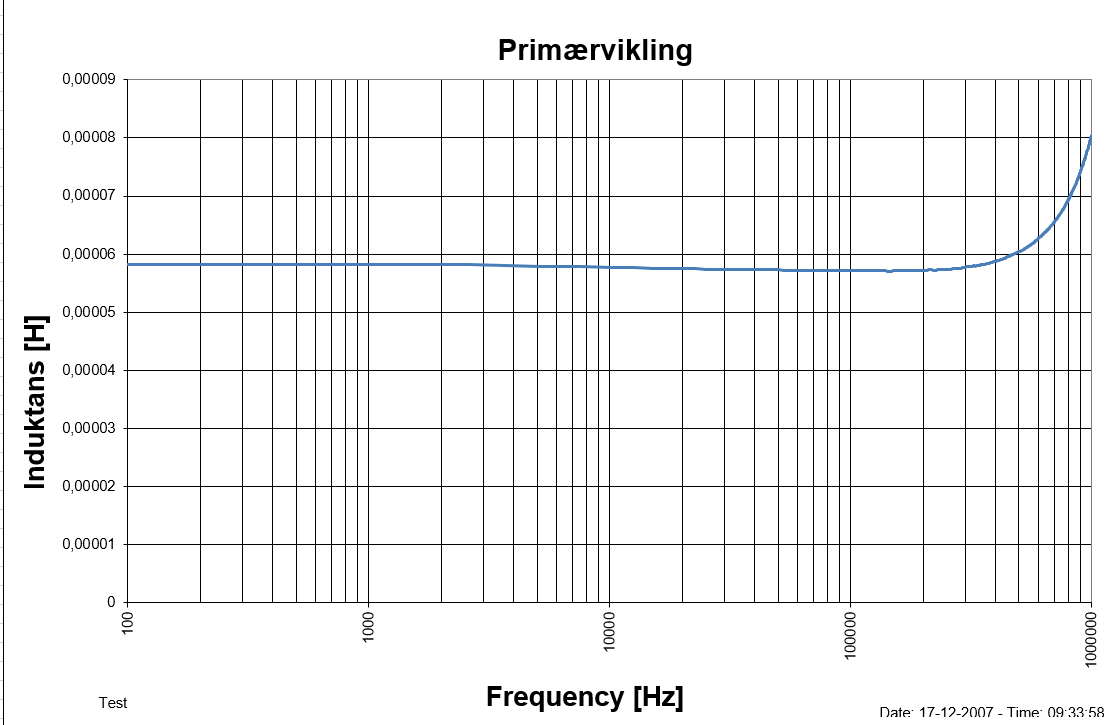
\includegraphics[max width=0.7\linewidth]{../dokumentation/tex/2iteration/billeder/Primarinduktans.png}
	\caption{Målt induktans i primær vikling}
	\label{fig: Primarinduktans}
\end{figure}
Ud fra de præcise værdier, som er vedlagt i bilagsmappen, findes induktansen ved 100kHz til $57.7\micro H$

Figur~\ref{fig: leakageinductance} viser spredningsselvinduktansen målt i transformatoren, ved et frekvenssweep på $100Hz$ til $1MHz$.
\begin{figure}[H]
	\center
	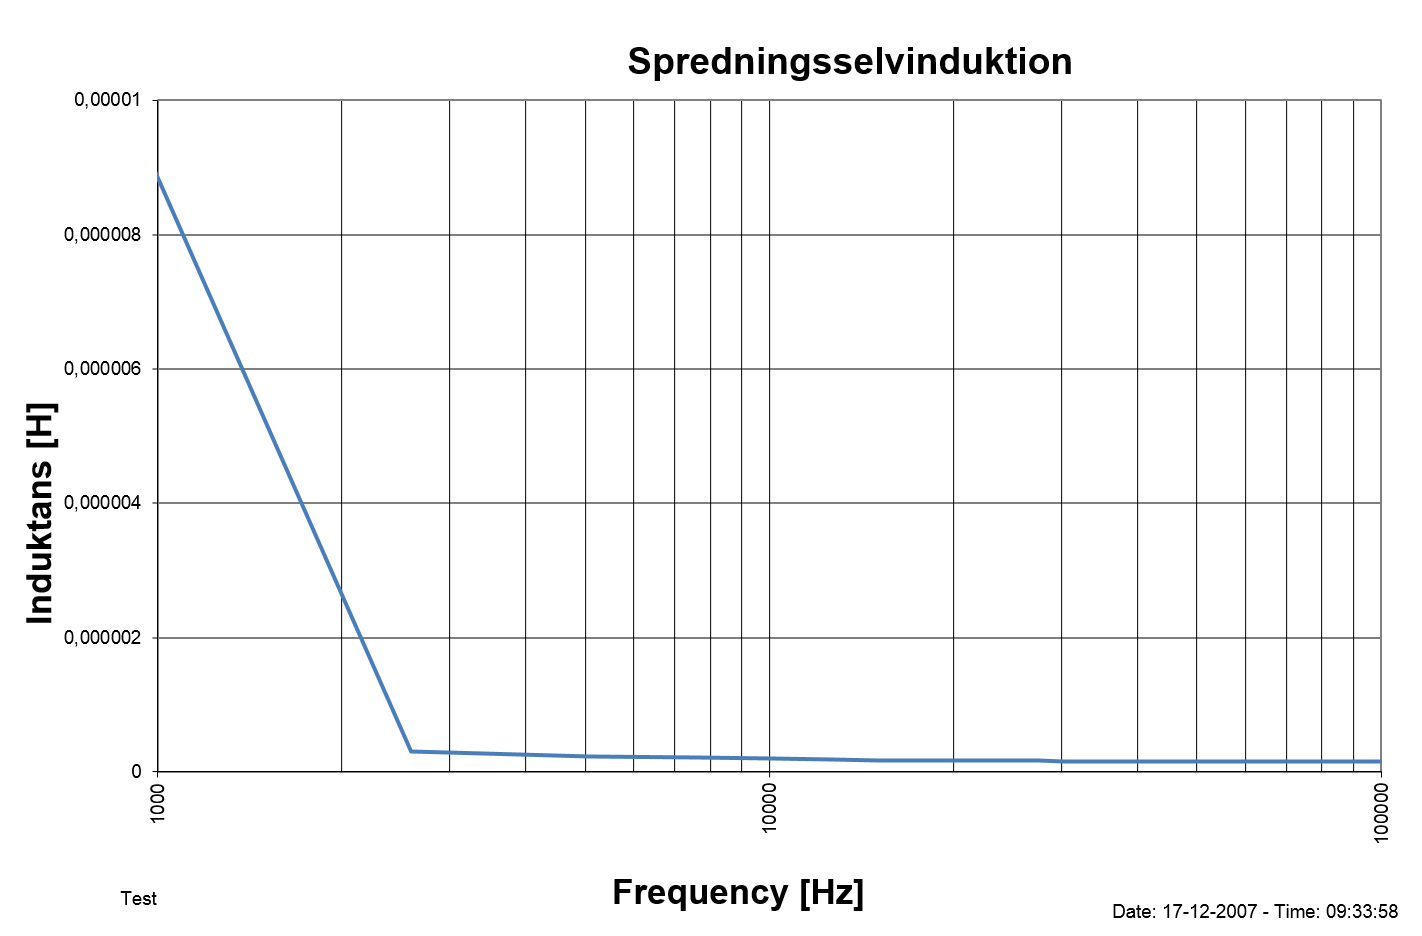
\includegraphics[max width=0.7\linewidth]{../dokumentation/tex/2iteration/billeder/Spredningsselvinduktion.png}
	\caption{Målt spredningsselvinduktion i transformator}
	\label{fig: leakageinductance}
\end{figure}

\subsection{Integrationtest - Constant load}
Figur~\ref{fig: Out26V} viser det realiserede spændingsoutput ved 26V. Kanal et viser spændingsoutputtet, mens kanal to viser gate spændingen for MOSFET'en. Kanal to er brugt til at trigge på, ved alle constant load målingerne. 
\begin{figure}[H]
	\center
	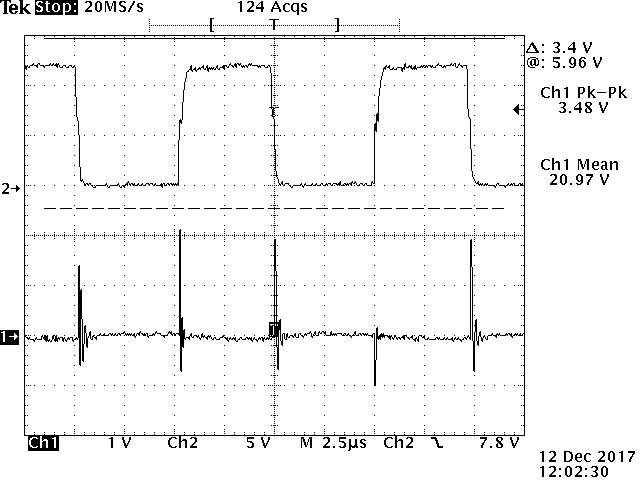
\includegraphics[max width=0.7\linewidth]{../dokumentation/tex/2iteration/billeder/Realisering/udgang_f_filter_2iteration.png}
	\caption{Spændingsoutput ved 26V}
	\label{fig: Out26V}
\end{figure}
Spændingen aflæses til at ligge på 20.97V. Yderligere observeres det, at der er swithing spikes på omkring 3.48V pk-pk.

Figur~\ref{fig: privolt} viser drain spændingen for MOSFET'en på kanal et, som også svarer til spændingen over den primære vikling i transformatoren.
\begin{figure}[H]
	\center
	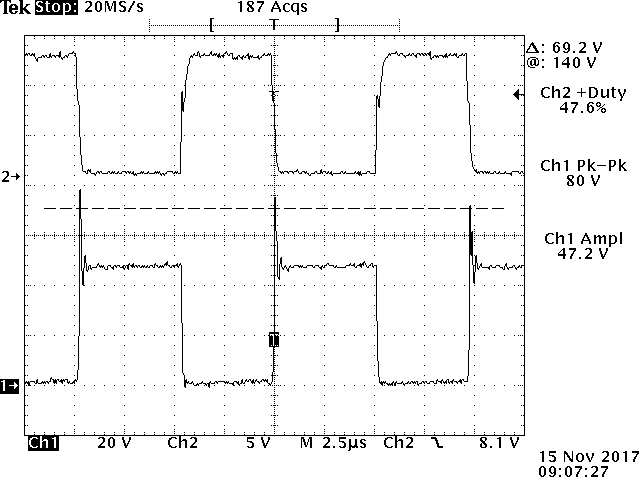
\includegraphics[max width=0.7\linewidth]{../dokumentation/tex/2iteration/billeder/Realisering/Transformator_Primar.png}
	\caption{Primær spænding}
	\label{fig: privolt}
\end{figure}
Spændingen over den primære vikling aflæses til en peak på 80V. Derudover aflæses den stationære spænding at ligge på 47V. 
På figur~\ref{fig: prizoom} er der zoomet ind på svingningerne omkring peakspændingen, som kunne observeres ovenfor.
\begin{figure}[H]
	\center
	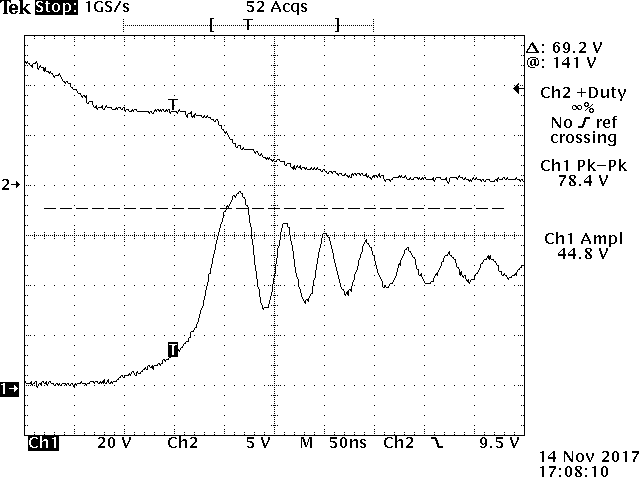
\includegraphics[max width=0.7\linewidth]{../dokumentation/tex/2iteration/billeder/Realisering/Transformator_Primarzoom.png}
	\caption{Zoomet på primær peak}
	\label{fig: prizoom}
\end{figure}
Svingningen for en periode aflæses til 40ns. Det svarer til en frekvens på $25MHz$

På figur~\ref{fig:sek} ses spændingen på anoden af dioden på kanal et, som også svarer til spændingen over den sekundære vikling.
\begin{figure}[H]
	\center
	\includegraphics[max width=0.7\linewidth]{../dokumentation/tex/2iteration/billeder/Realisering/Transformator_sekundar.png}
	\caption{Sekundær spænding}
	\label{fig:sek}
\end{figure}